\section{Ziel}
  Heutzutage ist es mit modernen Lasersystemen möglich ultrakurze Pulse im Bereich von wenigen Femtosekunden zu erzeugen und mit Hilfe dieser Prozesse mit Zeitskalen in der gleichen Größenordnung zu 
  untersuchen. Problematisch stellt sich dabei das Messen dieser ultrakurzen Pulsedar, weil die Messelektronik zu langsam arbeitet und nur Pulse bis zum niedrigen Nanosekundenbereich vermessen kann. In
  der Methode der Autokorrelation wird diese Limitierung umgangen, indem der fs-Puls mit sich selbst abgetastet wird und die Intensität bei jedem Abtastschritt über längere Zeit mit der vorhandenen 
  Elektronik gemessen werden kann. Solch ein Autokorrelator soll in diesem Versuch genutzt werden, um fs-Pulse sowie deren Verhalten beim Transmittieren durch Medien, wie Glas oder Silizium zu untersuchen.
    
\section{Theoretische Grundlagen}

  \subsection{Erzeugung ultrakurzer Pulse}
    Um Pulse mit Pulsdauern von wenigen Femtosekunden zu erzeugen werden Laser, die Licht mit einer besonders großen Bandbreite erzeugen, mit der Technik des Mode-Locking kombiniert. Die große Bandbreite
    $\Delta\nu$ ist dabei notwendig, da die zeitliche Dauer des Pulses $\Delta\tau$ durch die Heisenberg'sche Unschärferelation in Form des Zeit-Bandbreite-Produkts 
    
    \begin{equation}
      \Delta\tau \cdot \Delta\nu = \text{const},
    \end{equation}
    
    das eine von der Pulsform abhängige Konstante besitzt, nach unten limitiert ist.    


    \subsubsection{Mode-Locking}
      In dem Resonator eines Laser können für bis zu 100000 longitudinale Moden entstehen, die im Dauerstrich Laserbetrieb ohne feste Phasenbeziehung schwingen. Beim Mode-Locking wird versucht zwischen den 
      einzelnen Moden eine feste Phasenbeziehung zu erreichen, sodass es zu Interferenz zwischen den stehenden Wellen kommen kann. Dies führt, wie in Abbildung \ref{fig:Modelocking} a) zu sehen, zu einer 
      periodischen Wiederholung der Intensität mit der Durchlaufzeit durch den Resonator $T_C$. Zur Optimierung der Interferenz wird versucht die Phase aller Moden anzugleichen, sodass, wie in 
      Abbildung \ref{fig:Modelocking} b) dargestellt, letztendlich nur noch ein einzelnes ultrakurzes Wellenpaket durch den Resonator wandert und ausgekoppelt werden kann. Das Wellenpaket setzt sich also
      aus den stehenden Wellen der verschiedenen Frequenzen und kann als Fouriertransformation des Frequenzspektrums gesehen werden. Dies erklärt, dass die Menge der Moden und dementsprechend die 
      Bandbreite $\Delta\nu$ die minimal mögliche Pulsdauer $\Delta\tau_{\text{ML}}$ nach

      \begin{equation*}
        \Delta\tau_{\text{ML}} = \frac{2\pi}{\Delta\nu}
      \end{equation*}

      bestimmt. 
      Umgesetzt werden kann das Modelocking entweder durch die aktive Modulation, bei der zum Beispiel ein Shutter aktiv oszilliert, um längere Pulse abzuschwächen, oder durch passive Modulationen. In dem hier 
      genutzen System wird mit der Additiven Puls Modenkopplung eine passive Modulationsart genutzt. Diese beruht darauf, dass zunächst elliptisch polarisiertes Licht durch ein Medium läuft, dessen 
      Brechungsindex linear mit der Intensität des Lichts ansteigt. Dies führt zu einer Rotation der Ellipse, da die lineare Komponente der Ellipse mit der stärkeren Amplitude stärker zeitlich verzögert wird.

      \FloatBarrier
      \begin{figure}[h]
        \centering
        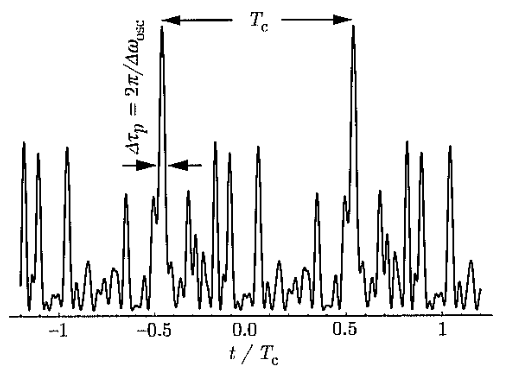
\includegraphics[width = 0.44\textwidth]{pictures/ML_phase_const.png}
        includegraphics[width = 0.44\textwidth]{pictures/ML_phase_gleich.png}
        \caption{a) Zeitlicher Verlauf der Intensität des Laser bei Überlagerung der Moden mit fester Phasenbeziehung. b)Zeitlicher Verlauf der Intensität, wenn die Moden alle die gleiche Phase besitzen. Entnommen aus \cite{tu_dortmund_versuchsanleitung_nodate}}
        \label{fig:Modelocking}
      \end{figure}
      \FloatBarrier
      
      
    \subsubsection{fs-Laser}
      Der in diesem Versuch genutzte Laser 
  
